\subsection{Funktionsweise}
Das Geiger-Müller-Zählrohr dient zu Intensitätsmessung ionisierender Strahlung.
Ein typischer Aufbau ist in Abbildung \ref{fig:aufbau} zu sehen.
\begin{figure}
  \centering
  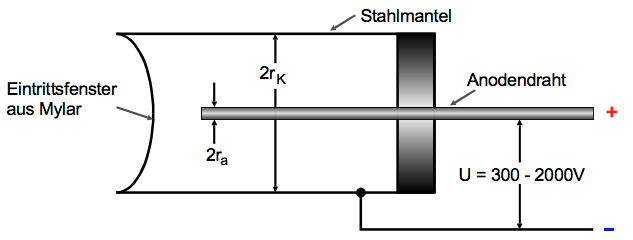
\includegraphics[width=0.8\textwidth]{bilder/aufbau.png}
  \caption{Aufbau des Geiger-Müller-Zählrohrs \cite{703}
  \label{fig:aufbau}}
\end{figure}
In der Mitte befindet sich ein Anodendraht mit Radius $r_\su{a}$ und außen herum
befindet sich ein Kathodenzylinder mit Radius $r_\su{k}$. Der gesamte Raum ist mit
einem Gasgemisch gefüllt. In diesem Raum wird ein elektrisches Feld
\begin{equation}
  E(r)= \frac{U}{r \cdot ln \bigg( \frac{r_\su{k}}{r_\su{a}}\bigg)}
\end{equation}
durch Anlegen einer Spannung von $U = (300-2000) \,\si{\volt}$ erzeugt, $r$
beschreibt den Abstand vom Anodendraht zum jeweiligen Punkt.
An der Stirnseite wird eine dünne Wand aus einem Material mit geringer Ordnungszahl
befestigt, z.B. eine Mylar-Folie, damit das Gas nicht austritt. Die $\alpha$ - Teilchen
können diese Folie jedoch problemslos durchdringen. Aufgrund eines Unterdrucks ist
die Folie leicht nach innen gewölbt. Man bezeichnet dies als Endfensterzählrohr.
Dringt nun ein Teilchen in das Zählrohr ein, so stößt es mit den Gasatomen zusammen
und ionisiert diese. Die frei werdenden Elektronen werden dann zum Anodendraht
beschleunigt. Die Spannung $U$ ist dann für den weiteren Verlauf entscheidend.
Die jeweiligen Fälle sind der Abb. \ref{fig:bereiche}
zu entnehmen.
\begin{figure}
  \centering
  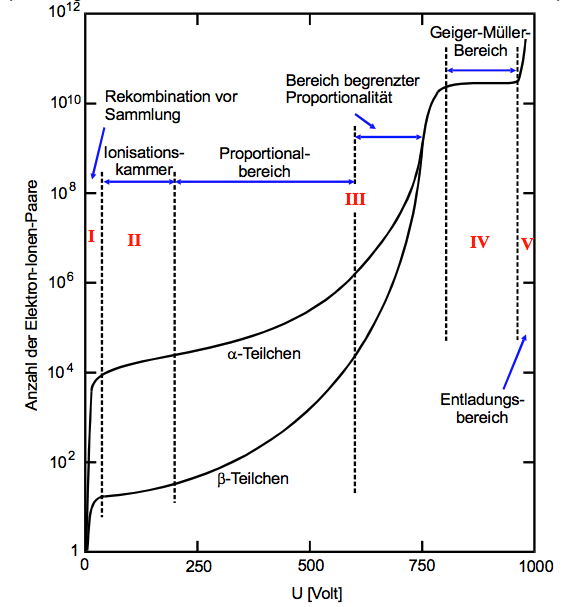
\includegraphics[width=10cm]{bilder/bereiche.png}
  \caption{Erzeugte Elektronenpaare in Abhängigkeit der Spannung U \cite{703}}
  \label{fig:bereiche}
\end{figure}
\begin{itemize}
  \item{I: Nur ein geringer Teil der Elektronen erreicht den Anodendraht.} \\
  \item{II: Nahezu alle Elektronen erreichen den Anodendraht. Es entsteht ein
  Ionisationsstrom, welcher proportional zur Energie und zur Intensität ist. Dies
  wird als Ionisationskammer bezeichnet. Aufgrund der geringen Ströme ist dieser Bereich
  nur für hohe Strahlungsintensitäten geeignet.} \\
  \item{III: Die Spannung ist hoch genug, damit die ausgelösten Elektronen weitere
  Stoßionisationen durchführen können. Es entsteht eine Townsend-Lawine. Die Ladung $Q$
  pro einfallendem Teilchen
  ist proportional zur Energie. Sie kann als Ladungsimpuls gemessen werden, wodurch
  in diesem Spannungsbereich, Porportionalzählrohr genannt, auch eine Engergiemessung
  möglich ist.} \\
  \item{IV: Die Spannung liegt über dem Proportionalitätsbereich. Die Ladung $Q$ ist
  unabhänging von der Primärionisation. In diesem Auslösebereich entstehen zusätzlich
  UV-Photonen, durch die Anregung der Gasatome. Diese breiten sich durch das gesamte
  Zählrohr aus und führen weitere Ionisationen durch. Die gemesse Ladung hängt somit
  nur noch von der Spannung und dem Gasvolumen ab. Dies ist der eigentliche Arbeitsbereich
  des Geiger-Müller-Zählrohrs. Er dient nur noch zur Intensitätsmessung.} \\
  \item{V: Dauerentladungen, welche das Zählrohr zerstören.}
\end{itemize}
Im Gegensatz zu den Elektronen aus den Stoßionisationen, wandern die positiven Ionen
nur sehr langsam zum Mantel. Dabei entsteht zeitweise ein positive Raumladung, welche
Stoßionisationen verhindert. Dieser Zeitraum wird als Totzeit $T$ bezeichnet. Während
der Wanderung der Ionen zum Mantel sinkt das positive Feld, wodurch wieder Ionisationen
möglich sind, jedoch nur mit einem geringerem Ladungsimpuls. Dies wird als Erholungszeit
$T_\su{E}$ bezeichnet. Siehe Abb. \ref{fig:totzeit}.
\begin{figure}
  \centering
  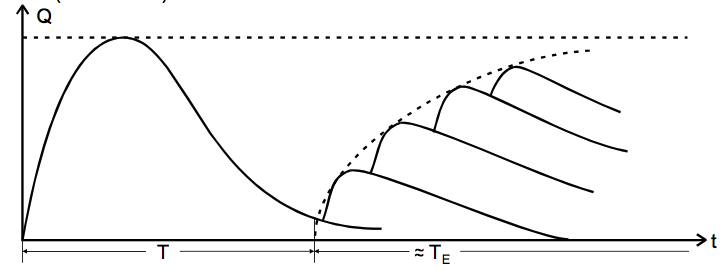
\includegraphics[width=0.8\textwidth]{bilder/totzeit.png}
  \caption{Totzeit und Erholungszeit eines Zählrohrs \cite{703}}
  \label{fig:totzeit}
\end{figure}
Beim Auftreffen der Ionen auf den Mantel werden weitere Elektronen ausgelöst, welche
dann erneut zum Anodendraht beschleunigt werden und dort einen Impuls auslösen. Dies
wird als Nachentladung bezeichnet. Die Laufzeit $T_\su{L}$ läuft also vom Austreten
des Elektrons aus dem Mantel, bis zum Ankommen an den Draht. Um diese Nachentladungen zu
unterdrücken werden Alkoholmoleküle zu dem Gasgemisch hinzugegeben. Die Ionen stoßen
dann nämlich mit den Alkoholmolekülen zusammen und ionisieren diese. Dadurch
wandern dann die Alkoholionen zum Mantel, jedoch reicht ihre Energie nicht aus, um dort
weitere Elektronen auszulösen.

\subsection{Charakteristik}
Die Charakteristik eines Zählrohrs ergibt sich durch das Auftragen der registrierten
Teilchenzahl $N$ gegen die angelegte Spannung $U$, bei konstanter Strahlungsintensität
(Siehe Abb. \ref{fig:plateau})
\begin{figure}
  \centering
  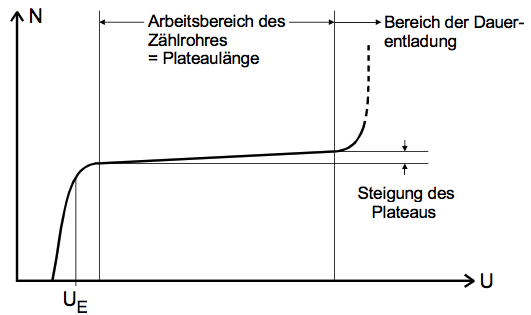
\includegraphics[width=0.6\textwidth]{bilder/plateau}
  \caption{Zählrohrcharakteristik \cite{703}}
  \label{fig:plateau}
\end{figure}
Ab der Spannung $U_\su{E}$ setzt der Auslösebereich ein. Der lineare Teil wird als
Plateau bezeichnet. Im Idealfall ist die Plateausteigung gleich Null. Aufgrund
einiger Nachentladungen ist dies jedoch in der Praxis nicht möglich. Die Länge und
Steigung des Plateaus ist auschlaggebend für die Qualität des Zählrohrs. Dem Plateau
schließt sich der Bereich der Dauerentladung an, welche durch ein einzelnes ionisierendes
Teilchen hervorgerufen werden kann.

\subsection{Ansprechvermögen}
Das Ansprechvermögen beschreibt die Wahrscheinlichkeit ein einfallendes Teilchen
nachzuweisen. Für $\alpha$ - und $\beta$ - Teilchen liegt das Ansprechvermögen bei
nahezu $100 \%$, aufgrund ihres hohen Ionisationsvermögens.
Für Photonen liegt das Ansprechvermögen dagegen bei nur ca. $1 \%$, da sie nur eine
sehr geringe Wechselwirkung mit Materie aufweisen. Dadurch kann das Geiger-Müller-Zählrohr
nur bei hohen $\gamma$ - Intensitäten sinnvol eingesetzt werden.
